% Propósito: comparar simultaneidad, enmascaramiento hacia adelante y hacia
% atrás mediante el orden temporal de la señal objetivo y el enmascarador.
% Origen: definiciones de la sección
% \ref{sec:u7-enmascaramiento-temporal}. Duraciones y separaciones
% esquemáticas; no representan ventanas temporales universales.
% Descripción accesible: tres líneas de tiempo muestran, respectivamente,
% objetivo y enmascarador superpuestos, enmascarador antes del objetivo y
% objetivo antes del enmascarador. En los dos últimos casos una flecha marca la
% separación temporal Delta t.
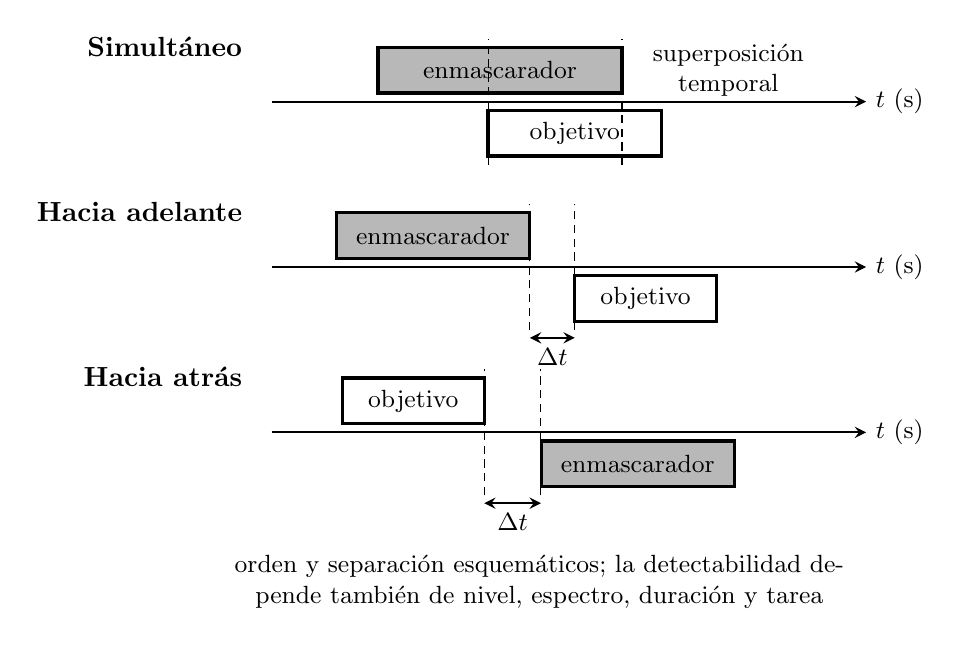
\begin{tikzpicture}[font=\small,>=stealth,x=1cm,y=1cm]
    \tikzset{
        masker/.style={draw,very thick,fill=black!28,minimum height=0.58cm},
        target/.style={draw,very thick,fill=white,minimum height=0.58cm}
    }

    \node[font=\bfseries,anchor=east] at (3.15,5.25) {Simultáneo};
    \draw[->,thick] (3.40,4.55) -- (10.95,4.55);
    \node[anchor=west] at (10.95,4.55) {\(t\) (s)};
    \node[masker,minimum width=3.10cm] at (6.30,4.95) {enmascarador};
    \node[target,minimum width=2.20cm] at (7.25,4.15) {objetivo};
    \draw[densely dashed] (6.15,3.75) -- (6.15,5.35);
    \draw[densely dashed] (7.85,3.75) -- (7.85,5.35);
    \node[align=center] at (9.20,4.95)
        {superposición\\temporal};

    \node[font=\bfseries,anchor=east] at (3.15,3.15)
        {Hacia adelante};
    \draw[->,thick] (3.40,2.45) -- (10.95,2.45);
    \node[anchor=west] at (10.95,2.45) {\(t\) (s)};
    \node[masker,minimum width=2.45cm] at (5.45,2.85) {enmascarador};
    \node[target,minimum width=1.80cm] at (8.15,2.05) {objetivo};
    \draw[densely dashed] (6.68,1.65) -- (6.68,3.25);
    \draw[densely dashed] (7.25,1.65) -- (7.25,3.25);
    \draw[<->,thick] (6.68,1.55) -- (7.25,1.55)
        node[midway,below] {\(\Delta t\)};

    \node[font=\bfseries,anchor=east] at (3.15,1.05)
        {Hacia atrás};
    \draw[->,thick] (3.40,0.35) -- (10.95,0.35);
    \node[anchor=west] at (10.95,0.35) {\(t\) (s)};
    \node[target,minimum width=1.80cm] at (5.20,0.75) {objetivo};
    \node[masker,minimum width=2.45cm] at (8.05,-0.05) {enmascarador};
    \draw[densely dashed] (6.10,-0.45) -- (6.10,1.15);
    \draw[densely dashed] (6.82,-0.45) -- (6.82,1.15);
    \draw[<->,thick] (6.10,-0.55) -- (6.82,-0.55)
        node[midway,below] {\(\Delta t\)};

    \node[align=center,text width=9.70cm] at (6.80,-1.55)
        {orden y separación esquemáticos; la detectabilidad depende también
         de nivel, espectro, duración y tarea};
\end{tikzpicture}
